\headline{\textbf{\Large\sffamily Bonsai Roots:}\\ 
         {\textbf{\large\sffamily Meet the Members of TWBC}}}
\label{2025-02-roots}
\noindent

Welcome to \emph{Bonsai Roots}, our monthly column where we shine a light on the people behind the trees.
This series is all about getting to know the members of the Twickenham Bonsai Club better and celebrating the diversity of experiences and stories that make our club so special.
This month, we're introducing \textbf{David Fishwick}!

\begin{itemize}
    \item \textbf{What's your name and where in the country do you live?}

    \emph{Hello, I'm David Fishwick. I live in Bordon, Hampshire.}

    \item \textbf{What are your favourite species of tree and why?}

    \emph{I have a special fondness for hawthorns. Their craggy bark gives them a timeless character, and I admire the way their thorns seem to defend them against whatever life throws their way-something I try to do myself.}

    \item \textbf{What aspect of bonsai do you enjoy?}

    \emph{Yamadori is my passion. I love the thrill and satisfaction of collecting trees from the wild.}

    \item \textbf{What aspects of bonsai do you find most challenging?}

    \emph{Patience. It's an art I've had to learn, but it's been an invaluable lesson both in bonsai and life.}

    \item \textbf{Who or what inspires you throughout your bonsai journey?}

    \emph{The Twickenham Bonsai Club itself has been a huge inspiration to me. The welcoming atmosphere and the collective passion of the members have not only made me a better bonsai enthusiast but also helped me focus and refine my approach to this art form.}

    \item \textbf{How long have you been interested in keeping bonsai?}

    \emph{I've been involved with bonsai for six years.}

    \begin{window}[%
        2,l,%
        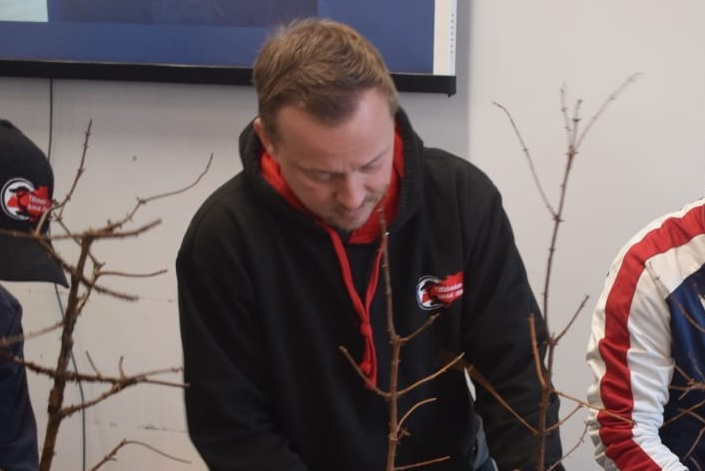
\includegraphics[width=1.0\columnwidth]{2025_02/res/roots_david_fishwick},%
        \centerline{\emph{Mark at work during a club workshop session.}}%
    ]
    \end{window}

    \item \textbf{What stimulated your interest in bonsai?}

    \emph{After losing my brother to suicide, I needed a way to break the negative cycle I found myself in. Bonsai became a way to heal and find peace.}

    \item \textbf{If you could give someone new to bonsai any tips, what would it be?}

    \emph{Learn the art of waiting. Patience is essential in bonsai and will serve you well in the long run.}

    \item \textbf{Why do you enjoy being part of TWBC, and do you have any ideas or suggestions for the club's future?}

    \emph{I love the club's modern format and how warmly I was welcomed into the Twickenham family. It's a truly special community.}

    \item \textbf{One word to describe what bonsai means to you?}

    \emph{Calming.}

    \item \textbf{What are your future goals regarding your own trees and learning more about the hobby?}

    \emph{I'd like to improve my trees to a level where they could be shown at exhibitions. I'm also keen to participate in one-to-one training sessions with some of the UK's top bonsai artists.}

    \item \textbf{How would you like to see your bonsai journey progress in the future?}

    \emph{My dream is to see one of my collected trees displayed in a top bonsai show.}
\end{itemize}

We hope you've enjoyed learning about David's inspiring journey.
Who will we meet next month?
Stay tuned for more from \emph{Bonsai Roots}!
\closearticle

%\vfill
\begin{center}
	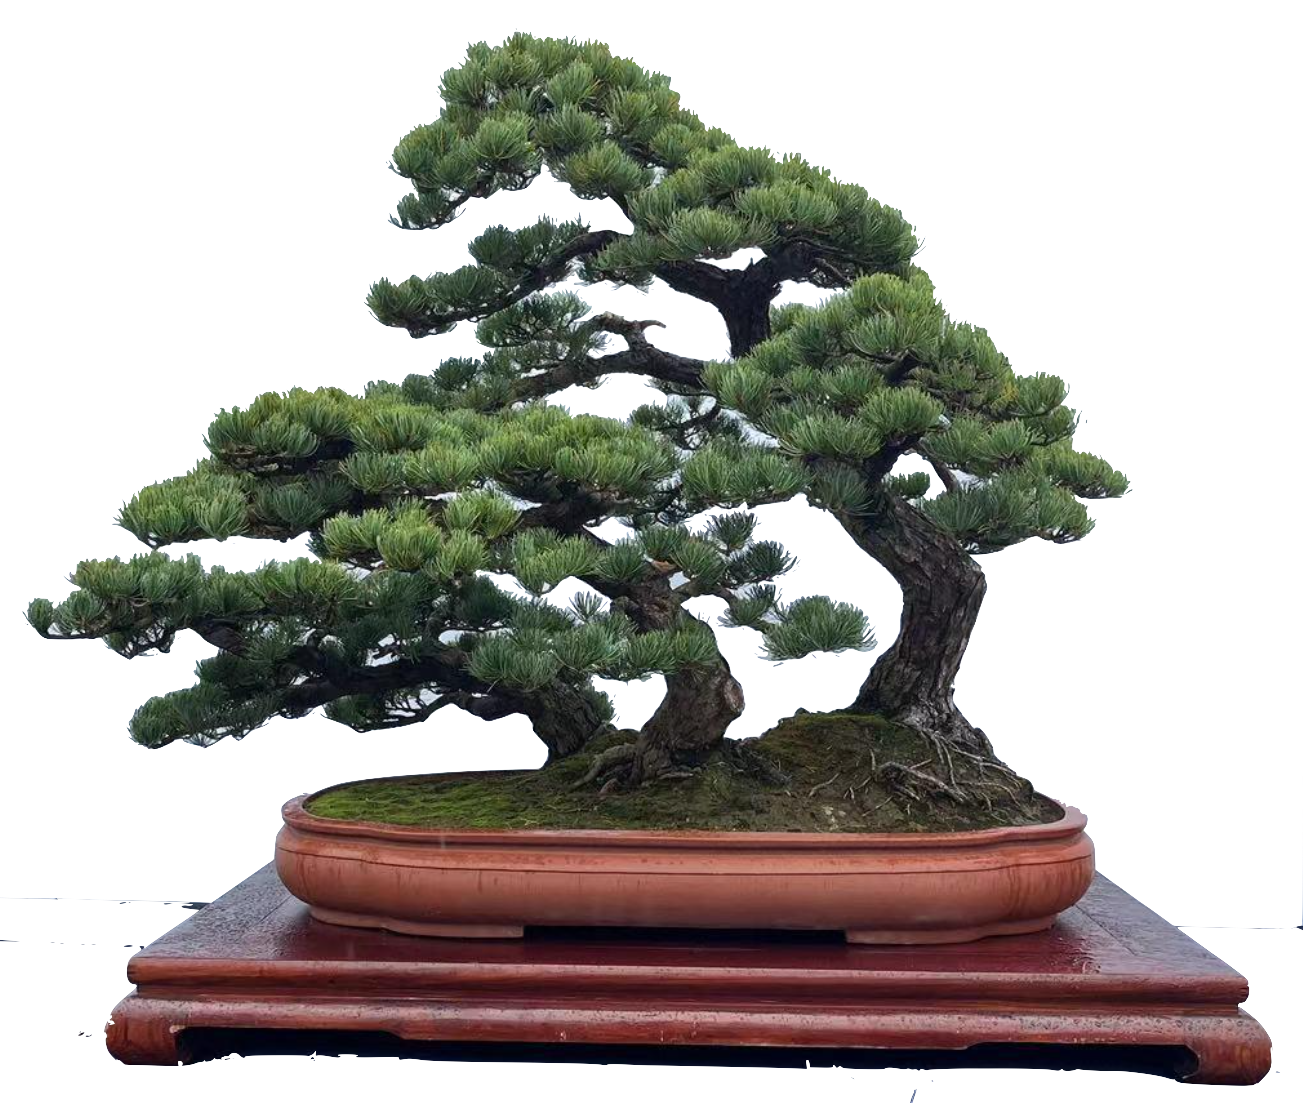
\includegraphics[width=0.8\columnwidth]{res/filler_a.png}
\end{center}
\columnbreak
